\section{Adfærd}
\label{sec:adfaerd}

De forskellige klasser og hændelser i problemområdet er nu blevet analyseret og beskrevet. Alle hændelsesforløb, der er mulige for alle objekter i en klasse, kan beskrives ved hjælp af adfærdsmønstre\cite[s.~90]{ooad}. Denne objektorienterede tilgang er baseret på, at der i vores systems model skal være et objekt for hvert objekt i problemområdet\cite[s.~91]{ooad}. Hvert objekt skal registrere og huske adfærden af det tilsvarende objekt i problemområdet, som det ændrer sig over tid.

\subsection{Indkøbsliste}
\label{subsec:brug-indkoebsliste}

Ud over muligheden for at tilføje opskrifternes ingredienser til indkøbslisten, så kan man også tilføje almindelig tekst til, så det er muligt at lave en indkøbsliste, der indeholder andet end ingredienser til madlavningen. Så man kan skrive andre varer på, som man kan købe med fra \fx supermarkedet. Systemets indkøbsliste kan ses i \figref{fig:overblik-indkoebsliste}.

\begin{figure}[H]
	\centering
	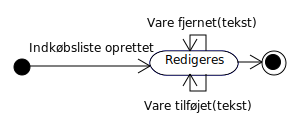
\includegraphics[scale=1]{billeder/foodl/thumbnails/indkoebsliste.png}
	\capt{Denne figur har til formål at give et overblik over systemets indkøbsliste.}
	\label{fig:overblik-indkoebsliste}
\end{figure}

Brugeren har mulighed for at tilføje varer i feltet ``tilføj til indkøbsliste'' og trykke på ``tilføj'' i bunden af siden. Der er mulighed for at slette alle varer fra indkøbslisten, ved at trykke på knappen ``slet alt'' i øverste højre hjørne af indkøbslisten, og ligeledes at slette enkelte varer, ved at trykke på de små gule krydser ud for alle varerne. Derudover er der implementeret en knap, til at udskrive indkøbslisten, som vi naturligvis kalder for ``udskriv''.

Hvis brugeren ikke er logget ind, vil de se i øverste højre hjørne af \figref{fig:overblik-indkoebsliste} (under sidehovedet) en boks, som informerer brugeren om, at man skal være logget ind for at systemet skal være i stand til at gemme indkøbslisten og favoritter. Oprettelse af bruger og indlogning bliver beskrevet nærmere i \secref{subsec:brug-opret}.

\subsection{Råvare}
Når nogen i sin husstand køber en råvare, indtræffer hændelsen \textit{råvare købt}. Denne hændelse fører råvare-klassen i en ny tilstand, der hedder \textit{brugbar}. Denne råvare er klar til at blive brugt. Inden der bliver handlet ind, og inden der sker et tilstandsskift, så er råvaren i en tidligere tilstand, der hedder \textit{eksisterer}. Dette tilstandsdiagram har ikke en afsluttendde hændelse, fordi vi har vurderet, at en råvare altid vil eksistere. Men den er først brugbar, når man har købt den. 

Indehaverne af en råvare har nu to muligheder. Man kan enten bruge hele råvaren, eller man ende med at smide noget af den ud. Disse to hændelser har vi samlet under en fælles hændelse, som vi kalder \textit{råvare opbrugt}. Denne hændelse fører klassen i en gammel tilstand, der hedder \textit{eksisterer}, da den ikke længere er brugbar i husstanden. Se \figref{fig:raavare-adfaerd}.

\begin{figure}[H]
	\centering
	\scalebox{0.8}{
	\subsection{Råvare}
Når nogen i sin husstand køber en råvare, indtræffer hændelsen \textit{råvare købt}. Denne hændelse fører råvare-klassen i en ny tilstand, der hedder \textit{brugbar}. Denne råvare er klar til at blive brugt. Inden der bliver handlet ind, og inden der sker et tilstandsskift, så er råvaren i en tidligere tilstand, der hedder \textit{eksisterer}. Dette tilstandsdiagram har ikke en afsluttendde hændelse, fordi vi har vurderet, at en råvare altid vil eksistere. Men den er først brugbar, når man har købt den. 

Indehaverne af en råvare har nu to muligheder. Man kan enten bruge hele råvaren, eller man ende med at smide noget af den ud. Disse to hændelser har vi samlet under en fælles hændelse, som vi kalder \textit{råvare opbrugt}. Denne hændelse fører klassen i en gammel tilstand, der hedder \textit{eksisterer}, da den ikke længere er brugbar i husstanden. Se \figref{fig:raavare-adfaerd}.

\begin{figure}[H]
	\centering
	\scalebox{0.8}{
	\subsection{Råvare}
Når nogen i sin husstand køber en råvare, indtræffer hændelsen \textit{råvare købt}. Denne hændelse fører råvare-klassen i en ny tilstand, der hedder \textit{brugbar}. Denne råvare er klar til at blive brugt. Inden der bliver handlet ind, og inden der sker et tilstandsskift, så er råvaren i en tidligere tilstand, der hedder \textit{eksisterer}. Dette tilstandsdiagram har ikke en afsluttendde hændelse, fordi vi har vurderet, at en råvare altid vil eksistere. Men den er først brugbar, når man har købt den. 

Indehaverne af en råvare har nu to muligheder. Man kan enten bruge hele råvaren, eller man ende med at smide noget af den ud. Disse to hændelser har vi samlet under en fælles hændelse, som vi kalder \textit{råvare opbrugt}. Denne hændelse fører klassen i en gammel tilstand, der hedder \textit{eksisterer}, da den ikke længere er brugbar i husstanden. Se \figref{fig:raavare-adfaerd}.

\begin{figure}[H]
	\centering
	\scalebox{0.8}{
	\input{billeder/tilstandsdiagrammer/raavare.pdf_tex}}
	\capt{Tilstandsdiagram for klassen råvare. De afrundede rektangulære bokse med tekst, skal anses som tilstande, som klassen kan have. De pile, der fører til en tilstand, skal anses som hændelser, som kan være skyld i et tilstandsskift. I dette tilfælde har klassen to tilstande (eksisterer) og (brugbar). Dette tilstandsdiagram har ikke en afsluttendde hændelse.}
	\label{fig:raavare-adfaerd}
\end{figure}}
	\capt{Tilstandsdiagram for klassen råvare. De afrundede rektangulære bokse med tekst, skal anses som tilstande, som klassen kan have. De pile, der fører til en tilstand, skal anses som hændelser, som kan være skyld i et tilstandsskift. I dette tilfælde har klassen to tilstande (eksisterer) og (brugbar). Dette tilstandsdiagram har ikke en afsluttendde hændelse.}
	\label{fig:raavare-adfaerd}
\end{figure}}
	\capt{Tilstandsdiagram for klassen råvare. De afrundede rektangulære bokse med tekst, skal anses som tilstande, som klassen kan have. De pile, der fører til en tilstand, skal anses som hændelser, som kan være skyld i et tilstandsskift. I dette tilfælde har klassen to tilstande (eksisterer) og (brugbar). Dette tilstandsdiagram har ikke en afsluttendde hændelse.}
	\label{fig:raavare-adfaerd}
\end{figure}
\subsection{Opskrift}
En opskrift kan befinde sig i en kogebog, på et stykke papir eller på en hjemmesiden. I \figref{fig:opskrift-adfaerd}, ses adfærden for klassen ``Opskrift''. En opskrift kommer til live, ved hændelsen \textit{opskrift fundet}. Her befinder den sig i tilstanden \textit{findes i opskriftssamlingen}. Hvis man er rigtig glad for en opskrift, kan man sætte et bogmærke på opskriften, så man hurtigt kan finde den igen. Sådan en hændelse kaldes for \textit{bogmærke tilføjet}. Hvis man ombestemmer sig og fjerner bogmærket, indtræffer hændelsen \textit{bogmærke fjernet}. Derudover kan man være nødsaget til at handle ind til en specifik opskrift, fordi man mangler nogle ingredienser. Det betyder, at man skal tilføje nogle opskrifter til en indkøbsliste. Denne hændelser kaldes for \textit{skrevet på indkøbsliste} med den modsignende hændelse \textit{fjernet fra indkøbsliste}. Der kan også eksistere en fejl i opskriften. En fejl kunne være et manglende billede til opskriften, eller at der står 20 minutter i ovnen i stedet for 40. Dette er beskrevet ved hjælp af hændelsen ``fejl fundet''. Disse fire hændelser medfører ikke et tilstandsskift. Opskriften ryger kun ud af tilstanden \textit{findes i opskriftssamlingen}, når opskriften fjernes, vha. hændelsen \textit{opskrift smidt ud}..

\pdffig[0.8]{tilstandsdiagrammer/opskrift}
  {Tilstandsdiagram for klassen opskrift. Klassen har én tilstand (findes i opskriftssamlingen) og en afsluttende hændelse ``opskrift fjernet'', der fører klassen ud i en sluttilstand.}
  {fig:opskrift-adfaerd}

\subsection{Bogmærke}
Som nævnt kan man vælge at tilføje et bogmærke til en opskrift, man kan lide. Denne hændelse kaldes \textit{bogmærke sat ind}, og bringer klassen i tilstanden \textit{aktiv}. Bogmærket er aktiv, indtil den kommer i sluttilstanden efter, at hændelsen \textit{bogmærke fjernet} indtræffer. Se \figref{fig:bogmaerke-adfaerd} for tilstandsdiagrammet over denne klasse.

\pdffig[0.8]{tilstandsdiagrammer/bogmaerke}
  {Tilstandsdiagram for klassen bogmærke. Klassen har én tilstand (aktiv) og en afsluttende hændelse ``bogmærke fjernet'', der fører klassen ud i sluttilstanden.}
  {fig:bogmaerke-adfaerd}

\subsection{Ingrediens}

\todo{Revider hele dette afsnit!}
En ingrediens kommer til verdenen sammen med en opskrift. Dette er fordi, at en ingrediens ikke er en del af problemområdet før den optræder i en opskrift. Det er nemlig først der, at man i en husstand behøver at bekymre sig om ingredienser. Hvis de ikke fandtes i nogle opskrifter, var der ikke nogen grund til at indkøbe en råvare svarende til ingrediensen, og ingrediensen ville derved ikke være en del af problemområdet. Denne hændelse kaldes \textit{Opskrift fundet}. Mens ingrediensen ekisister, er den i tilstanden af samme navn. Når man kender til en ingrediens, kan man skrive den på sin indkøbsliste. Dette gør man hvis man vil være sikre på at huske at købe en råvare svarende til ingrediensen, når man er ude at handle ind. Man kan selvfølgelig også fjerne ingrediensen fra sin indkøbsliste, hvis man har ombestemt sig og ikke ønsker at huskes på at købe den tilsvarende råvare. Disse to hændelser kaldes \textit{ingrediens tilføjet} og \textit{ingrediens fjernet}. Når opskriften, der indeholder en given ingrediens, smides ud, er hændelsen \textit{Opskrift smidt ud} netop indtruffet, og ingrediensen bringes i sin sluttilstand. Det bør bemærkes, at 2 forskellige opskrifter, der begge indeholder pasta, anses for at indeholde hver sin ingrediens. Dette er en vigtig adskillelse, da ingredienser består af en mængde og enhed, \fx 200 g pasta.

\begin{figure}[H]
	\centering
	\scalebox{0.6}{
	\subsection{Ingrediens}

\todo{Revider hele dette afsnit!}
En ingrediens kommer til verdenen sammen med en opskrift. Dette er fordi, at en ingrediens ikke er en del af problemområdet før den optræder i en opskrift. Det er nemlig først der, at man i en husstand behøver at bekymre sig om ingredienser. Hvis de ikke fandtes i nogle opskrifter, var der ikke nogen grund til at indkøbe en råvare svarende til ingrediensen, og ingrediensen ville derved ikke være en del af problemområdet. Denne hændelse kaldes \textit{Opskrift fundet}. Mens ingrediensen ekisister, er den i tilstanden af samme navn. Når man kender til en ingrediens, kan man skrive den på sin indkøbsliste. Dette gør man hvis man vil være sikre på at huske at købe en råvare svarende til ingrediensen, når man er ude at handle ind. Man kan selvfølgelig også fjerne ingrediensen fra sin indkøbsliste, hvis man har ombestemt sig og ikke ønsker at huskes på at købe den tilsvarende råvare. Disse to hændelser kaldes \textit{ingrediens tilføjet} og \textit{ingrediens fjernet}. Når opskriften, der indeholder en given ingrediens, smides ud, er hændelsen \textit{Opskrift smidt ud} netop indtruffet, og ingrediensen bringes i sin sluttilstand. Det bør bemærkes, at 2 forskellige opskrifter, der begge indeholder pasta, anses for at indeholde hver sin ingrediens. Dette er en vigtig adskillelse, da ingredienser består af en mængde og enhed, \fx 200 g pasta.

\begin{figure}[H]
	\centering
	\scalebox{0.6}{
	\subsection{Ingrediens}

\todo{Revider hele dette afsnit!}
En ingrediens kommer til verdenen sammen med en opskrift. Dette er fordi, at en ingrediens ikke er en del af problemområdet før den optræder i en opskrift. Det er nemlig først der, at man i en husstand behøver at bekymre sig om ingredienser. Hvis de ikke fandtes i nogle opskrifter, var der ikke nogen grund til at indkøbe en råvare svarende til ingrediensen, og ingrediensen ville derved ikke være en del af problemområdet. Denne hændelse kaldes \textit{Opskrift fundet}. Mens ingrediensen ekisister, er den i tilstanden af samme navn. Når man kender til en ingrediens, kan man skrive den på sin indkøbsliste. Dette gør man hvis man vil være sikre på at huske at købe en råvare svarende til ingrediensen, når man er ude at handle ind. Man kan selvfølgelig også fjerne ingrediensen fra sin indkøbsliste, hvis man har ombestemt sig og ikke ønsker at huskes på at købe den tilsvarende råvare. Disse to hændelser kaldes \textit{ingrediens tilføjet} og \textit{ingrediens fjernet}. Når opskriften, der indeholder en given ingrediens, smides ud, er hændelsen \textit{Opskrift smidt ud} netop indtruffet, og ingrediensen bringes i sin sluttilstand. Det bør bemærkes, at 2 forskellige opskrifter, der begge indeholder pasta, anses for at indeholde hver sin ingrediens. Dette er en vigtig adskillelse, da ingredienser består af en mængde og enhed, \fx 200 g pasta.

\begin{figure}[H]
	\centering
	\scalebox{0.6}{
	\input{billeder/tilstandsdiagrammer/ingrediens.pdf_tex}}
	\capt{Tilstandsdiagram for klassen ingrediens. I dette tilfælde har klassen én tilstand, nemlig eksisterer, og en afsluttende hændelse, der fører klassen ud i en sluttilstand.}
	\label{fig:ingrediens-adfaerd}
\end{figure}}
	\capt{Tilstandsdiagram for klassen ingrediens. I dette tilfælde har klassen én tilstand, nemlig eksisterer, og en afsluttende hændelse, der fører klassen ud i en sluttilstand.}
	\label{fig:ingrediens-adfaerd}
\end{figure}}
	\capt{Tilstandsdiagram for klassen ingrediens. I dette tilfælde har klassen én tilstand, nemlig eksisterer, og en afsluttende hændelse, der fører klassen ud i en sluttilstand.}
	\label{fig:ingrediens-adfaerd}
\end{figure}

